\documentclass[10pt, aspectratio=169]{beamer}

\usetheme[progressbar=frametitle]{metropolis}
\usepackage{appendixnumberbeamer}
\usepackage[round]{natbib}
\bibliographystyle{plainnat}

\usepackage{booktabs}
\usepackage[scale=2]{ccicons}

\usepackage{pgfplots}
\usepgfplotslibrary{dateplot}

\usepackage{xspace}
\newcommand{\themename}{\textbf{\textsc{metropolis}}\xspace}
\definecolor{specialgreen}{HTML}{14B03D}
\definecolor{specialblue}{HTML}{23373b}
\definecolor{specialorange}{HTML}{eb811b}




\title{Did the TCJA lower fiscal capacity of local jurisdictions?}
\date{\today}
\date{}
\author{Jakob Reinhardt}
\institute{Yale University}
% \titlegraphic{\hfill\includegraphics[height=1.5cm]{logo.pdf}}

\begin{document}

\maketitle

\begin{frame}{The TCJA and state/local fiscal capacity}
\begin{itemize}
    \item Tax Cuts and Jobs Act (\textbf{TCJA}) in 2017 overhauled the federal tax code.
    \begin{itemize}
        \item Largest reform of income tax code since Tax Reform Act (1986)
        \item Extensively analyzed, e.g. \cite{Chodorow-ReichSmithZidarZwick2025}, \cite{KennedyDobridgeLandefeldMortenson2025}, \cite{Chodorow-ReichZidarZwick2024}.
    \end{itemize}
    \vspace{.5cm}
    \item Capped \textbf{deductions} for state and local tax (\textbf{SALT}) deductions at \$10,000 for federal income taxes.
    \begin{itemize}
        \item Cut refunds for SALT by \textbf{\$90 Billion}
        \item Same order of magnitude as EITC, SNAP, Student Loan Programs.
    \end{itemize}
    \vspace{.5cm}
    \item End of subsidy was expected to increase \textbf{fiscal strain} on \textbf{local governments}. 
    \begin{itemize}
        \item Out-migration of high-income earners \citep{Tiebout1956}.
        \item Less public good provision (Education, Infrastructure, Public Safety).
    \end{itemize}
\end{itemize}    
\end{frame}


\begin{frame}{Contemporary Reactions}
    \begin{figure}
        \centering
        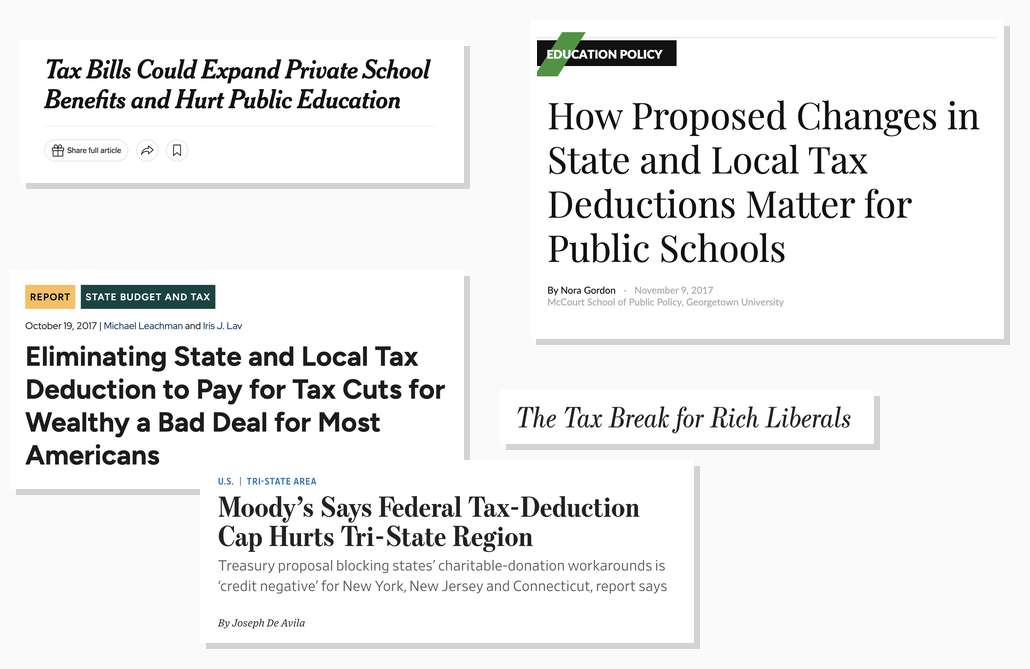
\includegraphics[width=0.8\linewidth]{figures/headline_collage.png}
        \label{fig:placeholder}
    \end{figure}
\end{frame}

\begin{frame}{This Paper}
    \begin{enumerate}
        \item Testing main predictions:
        \begin{itemize}
            \item Did \textbf{migration} from high-tax to low-tax states increase?
            \item Did \textbf{fiscal strain} on local government increase?
        \end{itemize}
        \vspace{.25cm}
        \item Data:
        \begin{itemize}
            \item IRS SOI county-level federal tax filings to construct policy exposure 
            \item IRS SOI county-to-county migration data.
            \item Annual Survey of State and Local Government Finances (ALFIN) for county-level sources of revenue.
            \item \textbf{Ideally: IRS/Census admin data.}
        \end{itemize}
        \vspace{.25cm}
        \item Research Design: Leveraging \textbf{spatial variation} in \textbf{policy exposure}
        \begin{itemize}
            \item Fit a gravity model to migration patterns and interact residuals with policy exposure.
        \end{itemize}
        \vspace{.25cm}
        \item Future work: Introduce a model of local public good provision with mobile taxpayers.
    \end{enumerate}
\end{frame}

\begin{frame}{Related literature}
    \begin{enumerate}
        \item \textbf{Evaluating} the \textbf{TCJA}
        \begin{itemize}
            \item Detailed evaluations in \cite{Chodorow-ReichSmithZidarZwick2025}, \cite{KennedyDobridgeLandefeldMortenson2025}, \cite{Chodorow-ReichZidarZwick2024} and  more.
            \item \cite{drukker}, \cite{YoungLurie2025}, \cite{Coen-PiraniSieg2019} and \cite{BruceKessler2022} on \textbf{migration}, \cite{Horton2023},  \cite{LiYu2022} and more on \textbf{housing markets}, \cite{AmbroseValentin2025} on \textbf{public good capitalization}.
            \item \alert{\textbf{Contribution:}} Evaluating effects on lower-level governments.
        \end{itemize}
        \vspace{.25cm}
        \item \textbf{Migration} responses to taxation: \cite{AkcigitBaslandzeStantcheva2016}, \cite{KlevenLandaisMunozStantcheva}, \cite{YoungVarnerLuriePrisinzano2016} and \cite{LiebigPuhaniSousa-Poza2007}
        \begin{itemize}
            \item \alert{\textbf{Contribution:}} Migration elasticities outside the top 1\% of earners.
        \end{itemize}
        \vspace{.25cm}
        \item {Public Finance} in a {spatial economy}
        \begin{itemize}
            \item Fiscal Federalism: \cite{Tiebout1956}, \cite{Oates1972}, \cite{Wilson1986}.
            \item Spatial Economics: \cite{Albouy2012}, \cite{FajgelbaumGaubert}, \cite{GaubertKlineVergaraYagan2025}.
        \end{itemize}
    \end{enumerate}
\end{frame}

\section{Insitutional Setting}

\begin{frame}{Federal income tax deductions reduce local effective tax rates}
    \metroset{block=fill}
    
    \begin{block}{\alert{Federal income tax}}
        \begin{itemize}
            \item Taxpayers subtract from adjustable gross income (AGI) the maximum of 
            \vspace{-.1cm}
            \begin{itemize}
                \item [a)] a flat \textbf{standard deduction} 
                \item[b)] \textbf{itemized} list of deductions $\rightarrow$ e.g. \textbf{SALT}, mortgages interest, charitable giving and more.
            \end{itemize}  
            \vspace{-.1cm}
            \item {If} itemizing, every \$1 spent on items has effective cost $1 - T^\prime(y)$.
            \vspace{-.1cm}
            \item Effective local tax rates vary across individuals:
            \vspace{-.1cm}
            $$\tau^{\text{eff}}_i = \begin{cases} \tau^{\text{statutory}} & \text{if not itemizing}_i \\ (1 - T'(y_i)) \cdot \tau^{\text{statutory}} & \text{if itemizing}_i \end{cases}$$
        \end{itemize}   
    \end{block}

    {\textbf{Changes} introduced by TCJA:}
    {\small
    \vspace{-.2cm}
    \begin{enumerate}
        \item {Standard deduction} increased roughly twofold.
        \begin{itemize}
            \item[$\rightarrow$] Fewer people itemize and effective local tax rates increase.
        \end{itemize}
        \item {SALT} deduction cap of \$10,000.
        \begin{itemize}
            \item[$\rightarrow$] Itemizers who are capped face higher effective \textit{marginal} rates.
        \end{itemize}
    \end{enumerate}
    }

\end{frame}


\begin{frame}{State and local tax deductions plummet post TCJA}
    \vspace{.25cm}
    \renewcommand{\thefootnote}{}%
    \footnotetext{Source: IRS SOI Historic Table 2, items N1, N04470, N18425 and N18500.}%
    \renewcommand{\thefootnote}{\arabic{footnote}}
    \begin{figure}
        \centering
        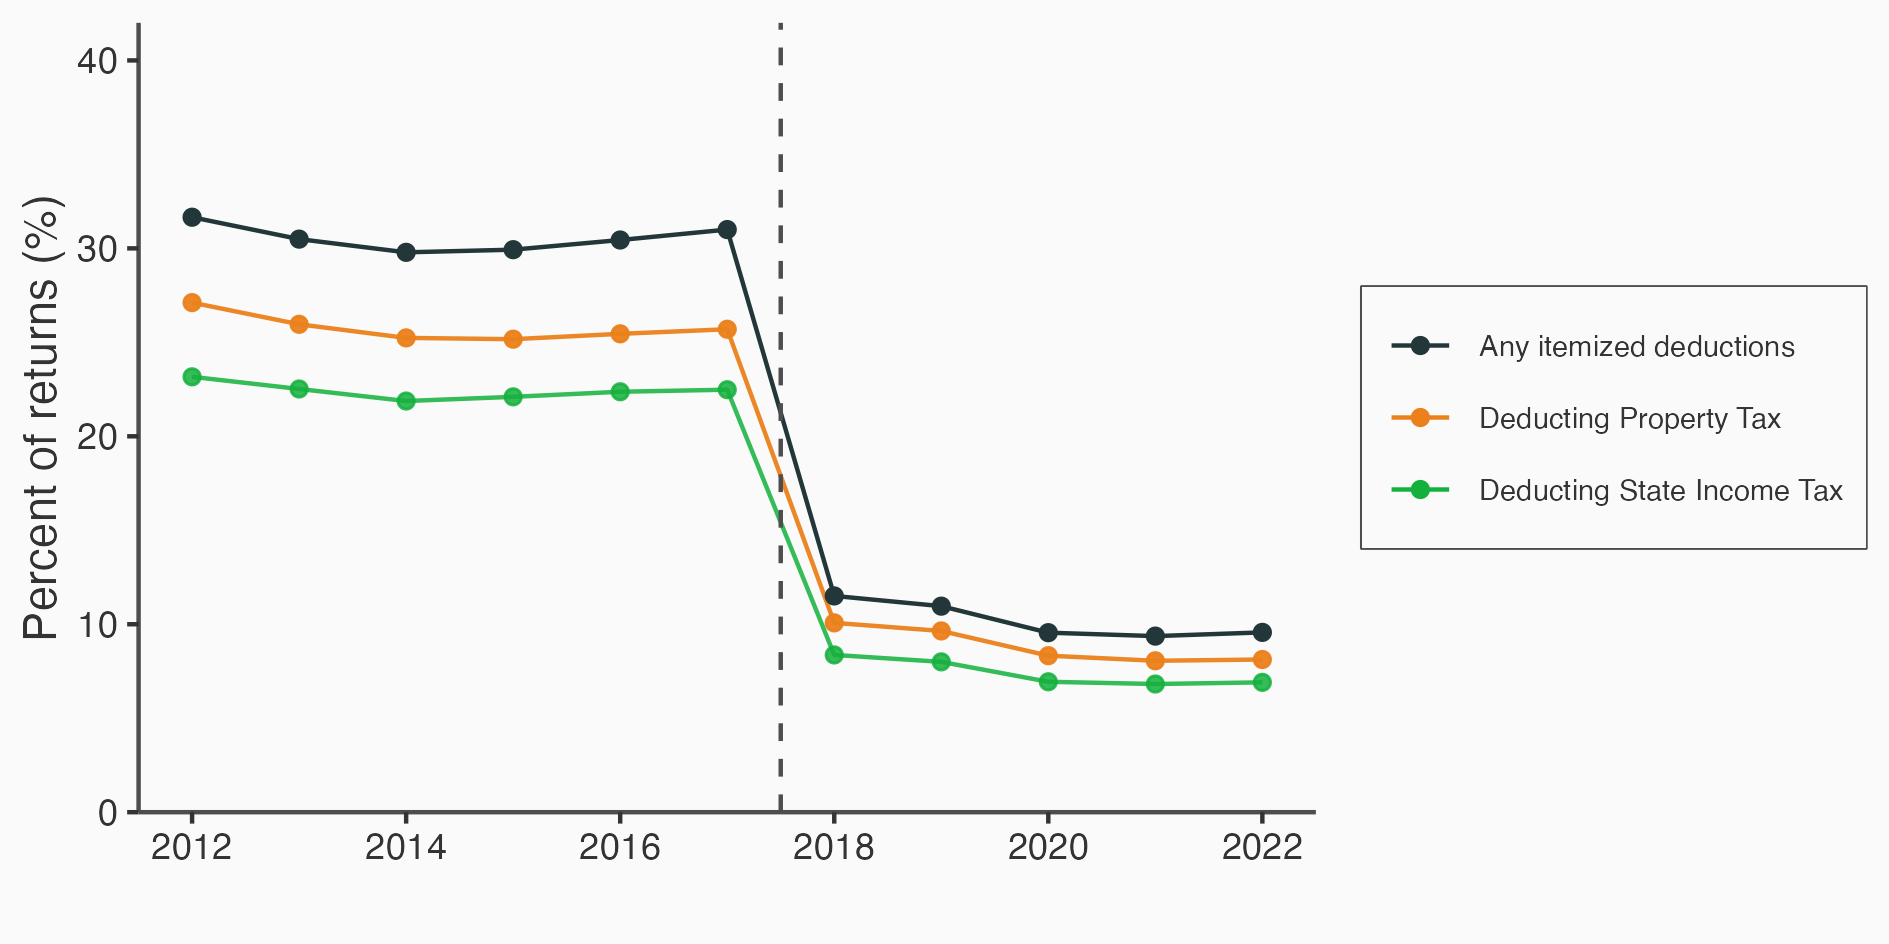
\includegraphics[width=.95\linewidth]{figures/fig1.png}
    \end{figure}
\end{frame}

\begin{frame}{A good setting to study local public good provision}

    \begin{block}{\textbf{Advantages:}}
        \begin{enumerate}
            \item Variation in \textbf{costs} of providing local public goods but held spending constant.
            \begin{itemize}
                \item[$\rightarrow$] Most literature focuses on spending \textbf{and} cost increases (e.g. \cite{BayerBlairWhaley2023}).
            \end{itemize}
            \item Large increase with lots of variation across \textbf{space} and \textbf{income}.
            \begin{itemize}
                \item[$\rightarrow$] Effective local tax rates increased by up to 58\%!
                \item[$\rightarrow$] Share of households exposed between 2\% and 58\% at the zipcode level.
            \end{itemize}
        \end{enumerate}

        \begin{block}{Disadvantages}
            \begin{itemize}
                \item Publicly available data necessitates using spatial variation
                \begin{itemize}
                    \item[$\rightarrow$] Other TCJA effects correlated with treatment assignment across space?
                \end{itemize}
                \item Some states introduced legislation to circumvent cap.
            \end{itemize}
        \end{block}
        
    \end{block}
    
    
    
    
\end{frame}

\section{Impact on Migration}

% Assumptions: 
% - SALT is constant
% - Itemization is constant within each regime
% - Monotonicity in itemization
% - No jumping across marginal tax rate brackets
% - No workarounds like NY, CA, etc.
\begin{frame}{Research Design: Gravity model}
    \textbf{Challenge:} Taxfilers increasingly migrate towards low-SALT states from 2011-2022.\\
    \vspace{.5cm}
    \textbf{Assume} migration flows between counties follow a gravity equation, including controls for state tax differentials:
    $$Mig_{ijt} = \alpha \cdot log(Pop_{it}) + \beta \cdot log(Pop_{jt}) + \delta \cdot log(Dist_{ij}) + X_{ijt}^\prime \gamma + \alert{\theta_t\Delta SALT_{ij}} + \epsilon_{ijt}$$
    where $i$, $j$ are counties, $t$ is time, $X_{ijt}$ is the baseline difference in average SALT between counties and $\Delta SALT_{ij}$ is the change in effective SALT paid across counties due to TCJA.\\
    \vspace{.5cm}
    \textbf{Identification:}
    \begin{itemize}
        \item Treatment isolates variation in itemization rates conditional on the level of SALT.
        \item ``Strong'' parallel trends required \citep{CallawayGoodman-BaconSantanna2024}
    \end{itemize}

\end{frame}

\begin{frame}{Data: County-level publicly available IRS/Census data}
    \begin{enumerate}
        \item County-to-county \textbf{migration rates} are taken from the IRS SOI. 
        \begin{enumerate}[a)]
            \item Includes average AGI of those moving.
        \end{enumerate}
        \item \textbf{Population} estimates are from the 5-year ACS.
        \item Differences in (effective) \textbf{SALT} across counties and TCJA-induced changes:
        \begin{enumerate}[a)]
            \item IRS SOI provide itemized SALT totals on the county-level by AGI-bins.
            \item Impute average marginal tax rate by filer type in each AGI bin.
            \item Using AGI-specific itemization rates, impute effective SALT paid per county per year.
            \item Policy exposure \alert{$\Delta SALT$} is the 2017-2018 change.
        \end{enumerate}
    \end{enumerate}
\end{frame}

\begin{frame}{Exposed taxfilers moved into lower-SALT counties.}
    
    \metroset{block=fill}
    \begin{alertblock}{\textbf{Model}:}
        $$Mig_{ijt} = \alpha \cdot log(Pop_{it}) + \beta \cdot log(Pop_{jt}) + \delta \cdot log(Dist_{ij}) + X_{ijt}^\prime \gamma + \alert{\theta_t \cdot \Delta SALT_{ij}} + \epsilon_{ijt}{ijt}$$
    \end{alertblock}
    \vspace{-.3cm}
    
    \begin{columns}[T]
        \begin{column}{0.6\textwidth}
            \begin{figure}
                \centering
                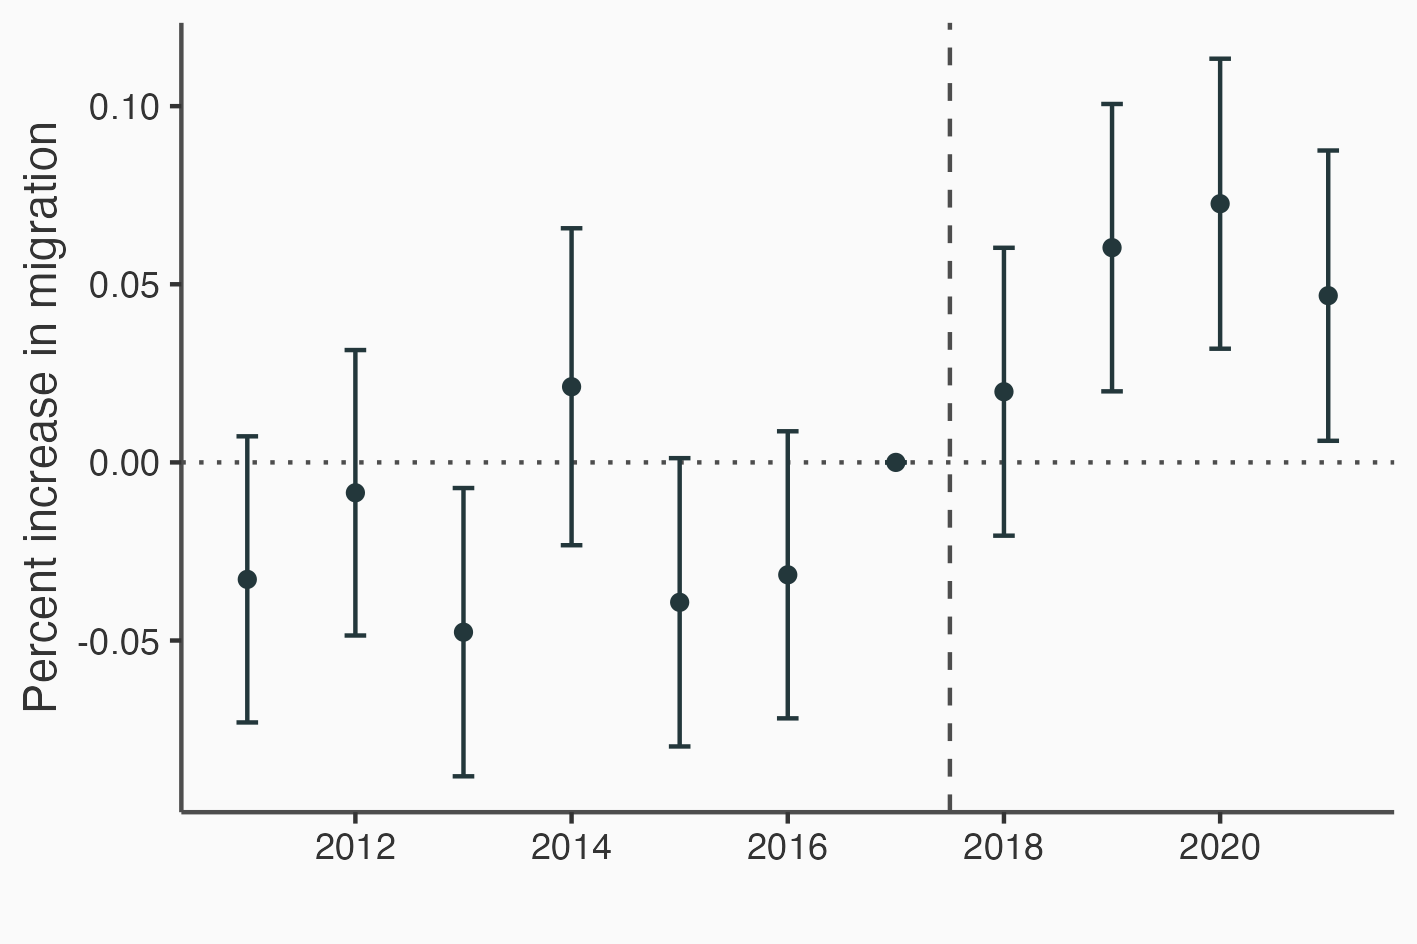
\includegraphics[width=\linewidth]{figures/fig_gravity_event_study.png}
                \label{fig:placeholder}
            \end{figure}
        \end{column}
        \begin{column}{0.4\textwidth}
            \vspace{.5cm}
            \begin{enumerate}
                \item Effect size: A 1\% change in SALT paid leads to a 0.15\% change in migration.
                \vspace{.15cm}
                \item Much lower than previous tax-induced migration estimates.
                \vspace{.15cm}
                \item Mirrors finding in \cite{YoungLurie2025} for millionaire taxpayers.
            \end{enumerate}
        \end{column}
    \end{columns}
\end{frame}

%\item Denoting itemization as $\mathcal{I}_{it}$, marginal federal income tax rate as $T^\prime_i$ and 
%\item $\mathcal{I}_{it}$ itemization dummy. Suppose $\mathcal{I}_{it}$ is constant in each pre/post reform regime.
%       \begin{itemize}
%          \item[$\Rightarrow$] $\Delta \mathcal{I}_{i} = \mathcal{I}_i^{post} - \mathcal{I}_i^{pre}$, $\Delta \mathcal{I}_{i} \in \{-1, 0\}.$
%\end{itemize}
%\item $\Delta T^{local}_{it} = \Delta\mathcal{I}_i\cdot T^\prime(y_i)\cdot SALT$

% \begin{frame}{Fewer taxfilers moved into exposed, high-tax states}
%     \begin{figure}
%         \centering
%         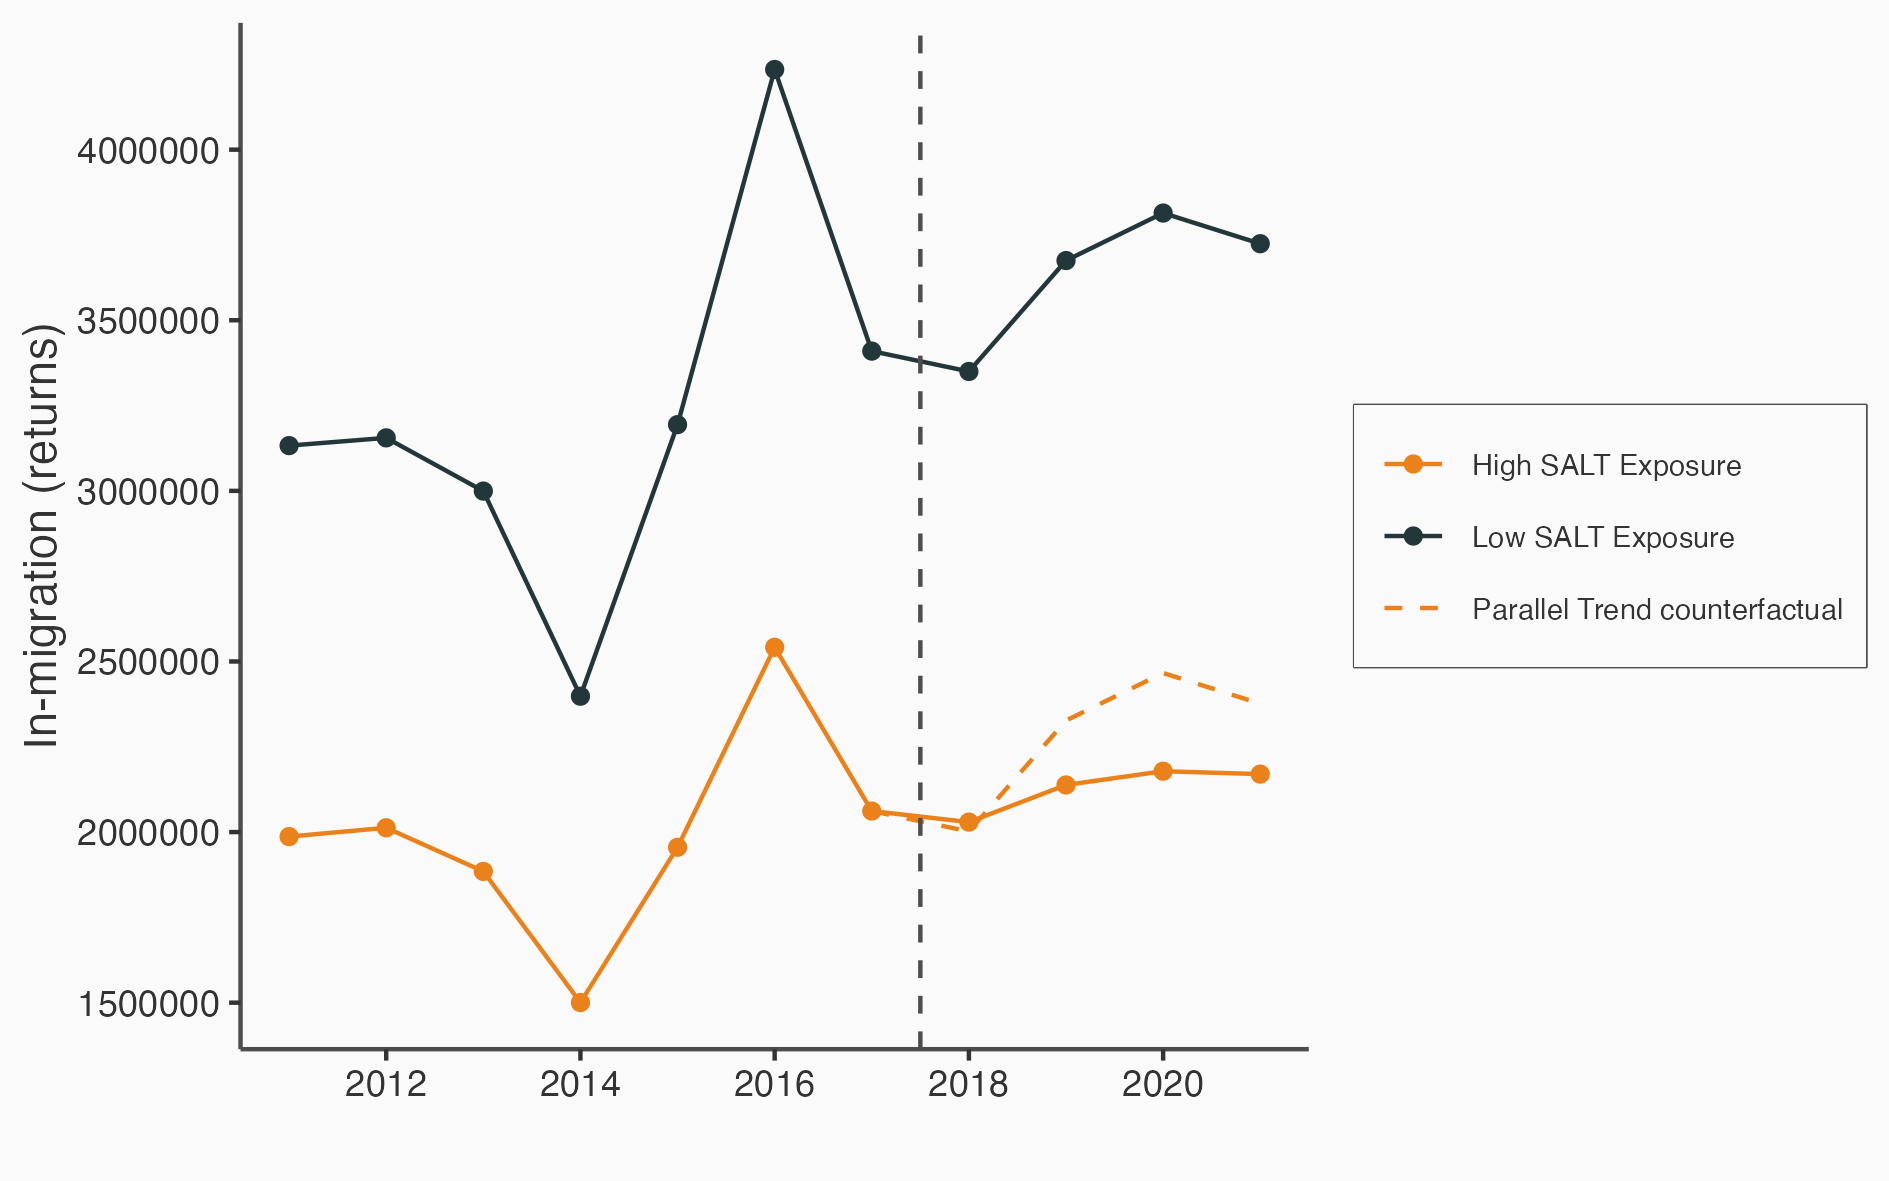
\includegraphics[width=0.8\linewidth]{figures/fig2.png}
%         \label{fig:placeholder}
%     \end{figure}
% \end{frame}

% \begin{frame}{Fewer taxfilers moved into exposed, high-tax states}

%     \metroset{block=fill}

%     \begin{alertblock}{\textbf{Model}:}
%         $$Migration_{ijt} = \alpha_{ij} + \delta_t + \beta_tD_{ijt} + \epsilon_{ijt}$$
%     \end{alertblock}
%     \vspace{-.3cm}
%     \begin{figure}
%         \centering
%         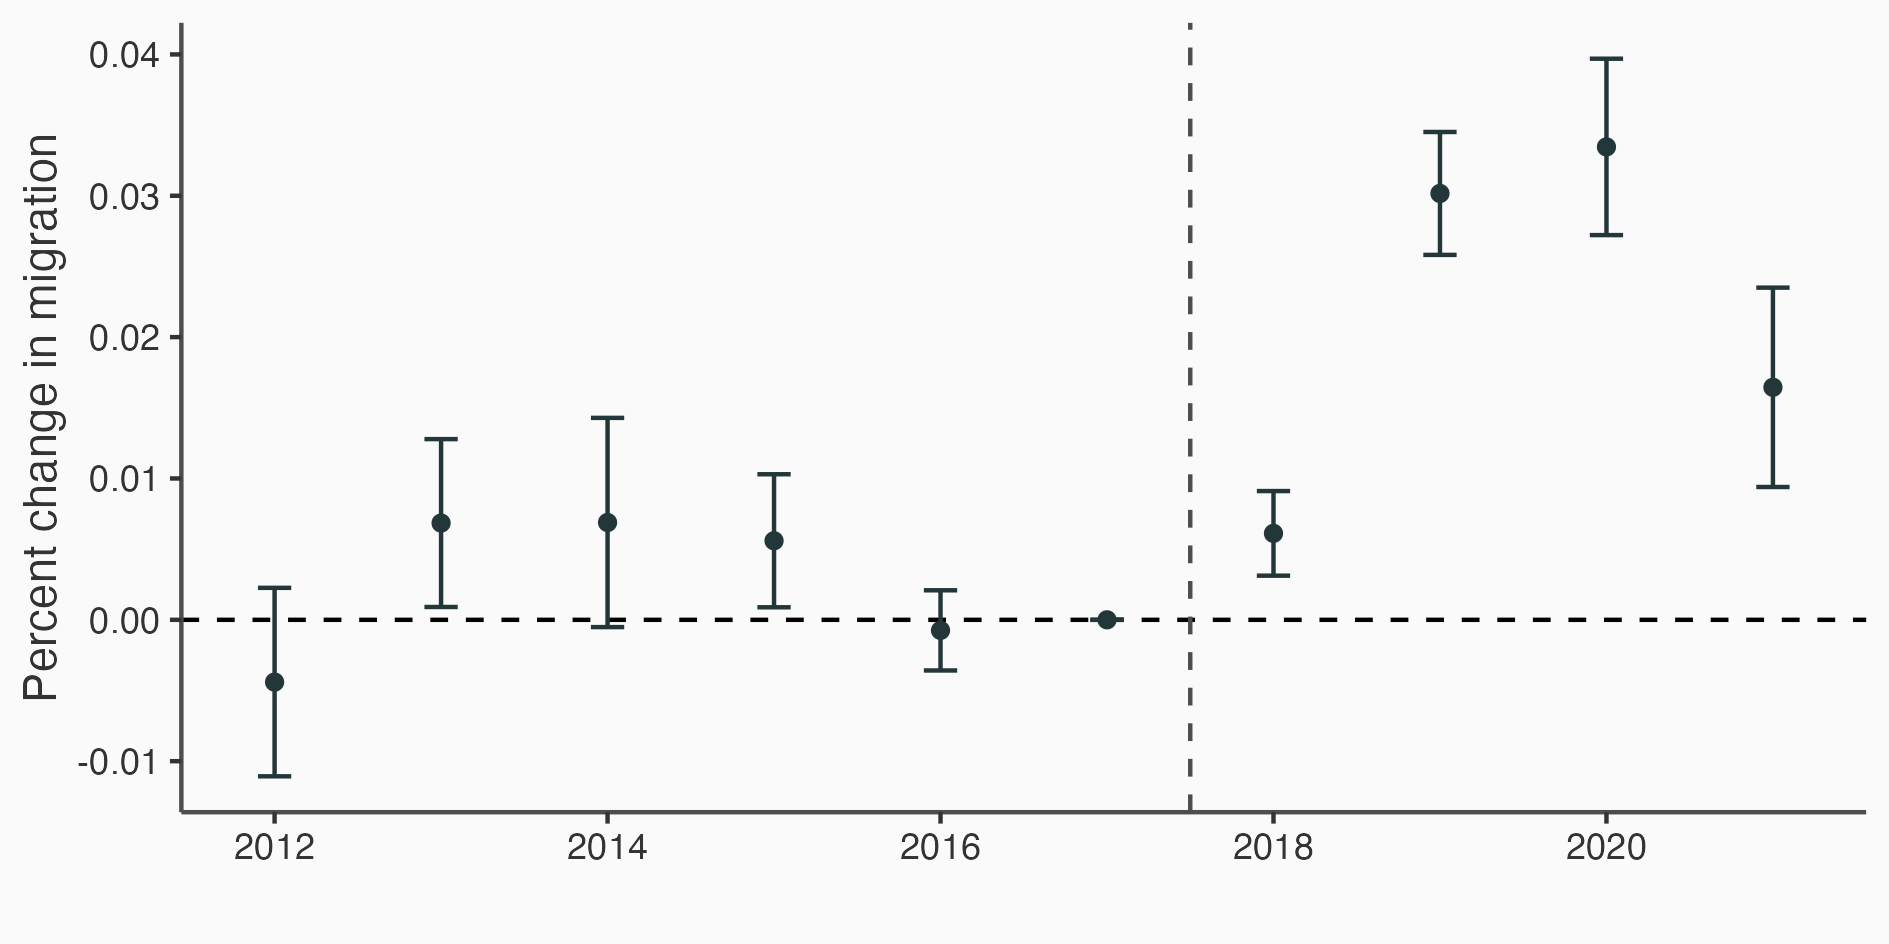
\includegraphics[width=0.75\linewidth]{figures/fig3.png}
%         \label{fig:placeholder}
%     \end{figure}
% \end{frame}


\begin{frame}{Average AGI of movers in exposed states increased}

    \metroset{block=fill}

    \begin{alertblock}{\textbf{Model}:}
        $$AGI_{ijt} = \alpha_{ij} + \delta_t + \alert{\theta_t\Delta SALT_{ijt}} + \epsilon_{ijt}$$
    \end{alertblock}
    \vspace{-.3cm}
    \begin{figure}
        \centering
        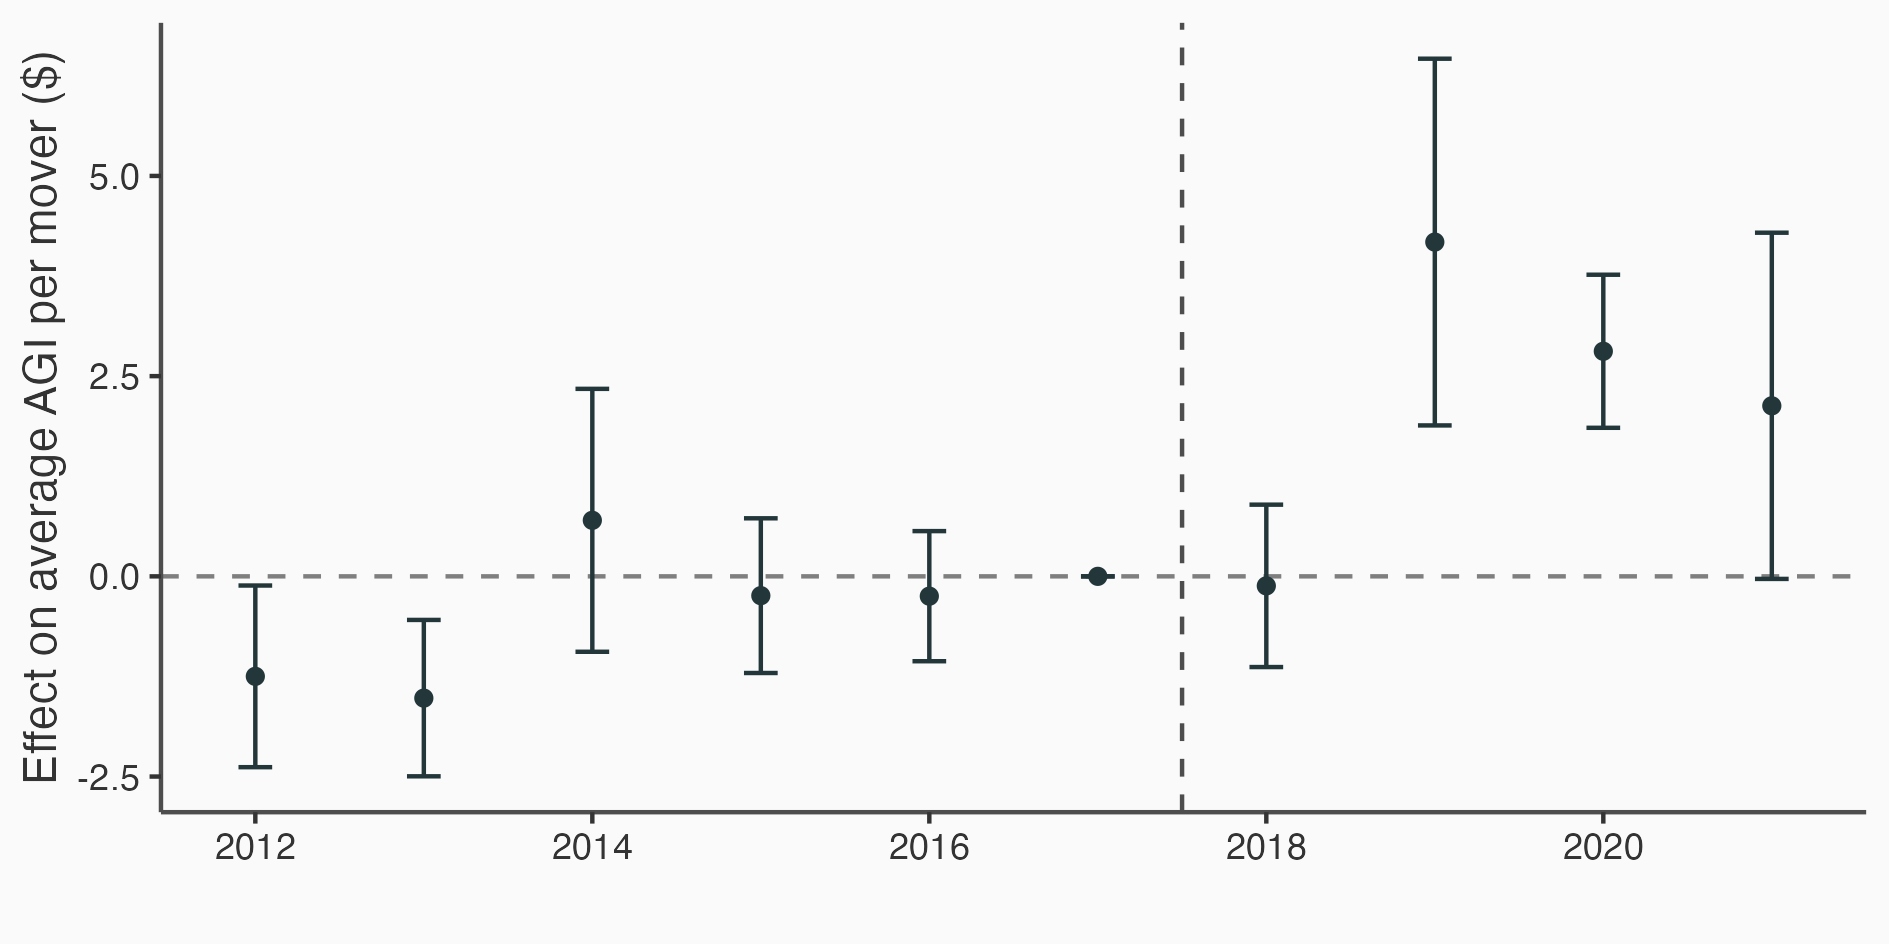
\includegraphics[width=0.75\linewidth]{figures/fig4.png}
        \label{fig:placeholder}
    \end{figure}
\end{frame}

\section{Impact on local finances}

\begin{frame}{Data and Research Design: NCES and Diff-in-Diff}
    \begin{enumerate}
        \item \textbf{Data}:
        \begin{itemize}
            \item ALFIN contains annual survey responses from a sample of local gov'ts. 
            \item Full census of all 90,000 local gov'ts every 5 years.
            \item Information on revenue by source, gov't employees and compensation, education expenditure and more.
        \end{itemize}
        \item \textbf{Research Design}:
        \begin{itemize}
            \item Leverage change in effective $SALT_{it}$ paid pre- vs. post-TCJA. 
            \item Assume local government spending has two-way-fixed effect structure.
            \item Restriction: Local gov't average spending only changes because of common state/federal-level shocks.
        \end{itemize}
        \item \textbf{Model:}
        $$log(y_{it}) = \alpha_i + \beta_t + \alert{\theta_t \cdot SALT_{it}} + \epsilon_{it}$$
        where $y_{it}$ is revenue for county $i$ at time $t$. Requires strong parallel trends \citep{CallawayGoodman-BaconSantanna2024} for interpretation as a postively-weighted average marginal treatment effect.
    \end{enumerate}
\end{frame}

\begin{frame}{Exposed counties lose revenue}
    \metroset{block=fill}
    \begin{alertblock}{\textbf{Model}:}
        $$log(y_{it}) = \alpha_i + \beta_t + \alert{\theta_t \cdot SALT_{it}} + \epsilon_{it}$$
    \end{alertblock}
    \vspace{-.3cm}
    
    \begin{columns}[c]
        \begin{column}{0.6\textwidth}
            \begin{figure}
                \centering
                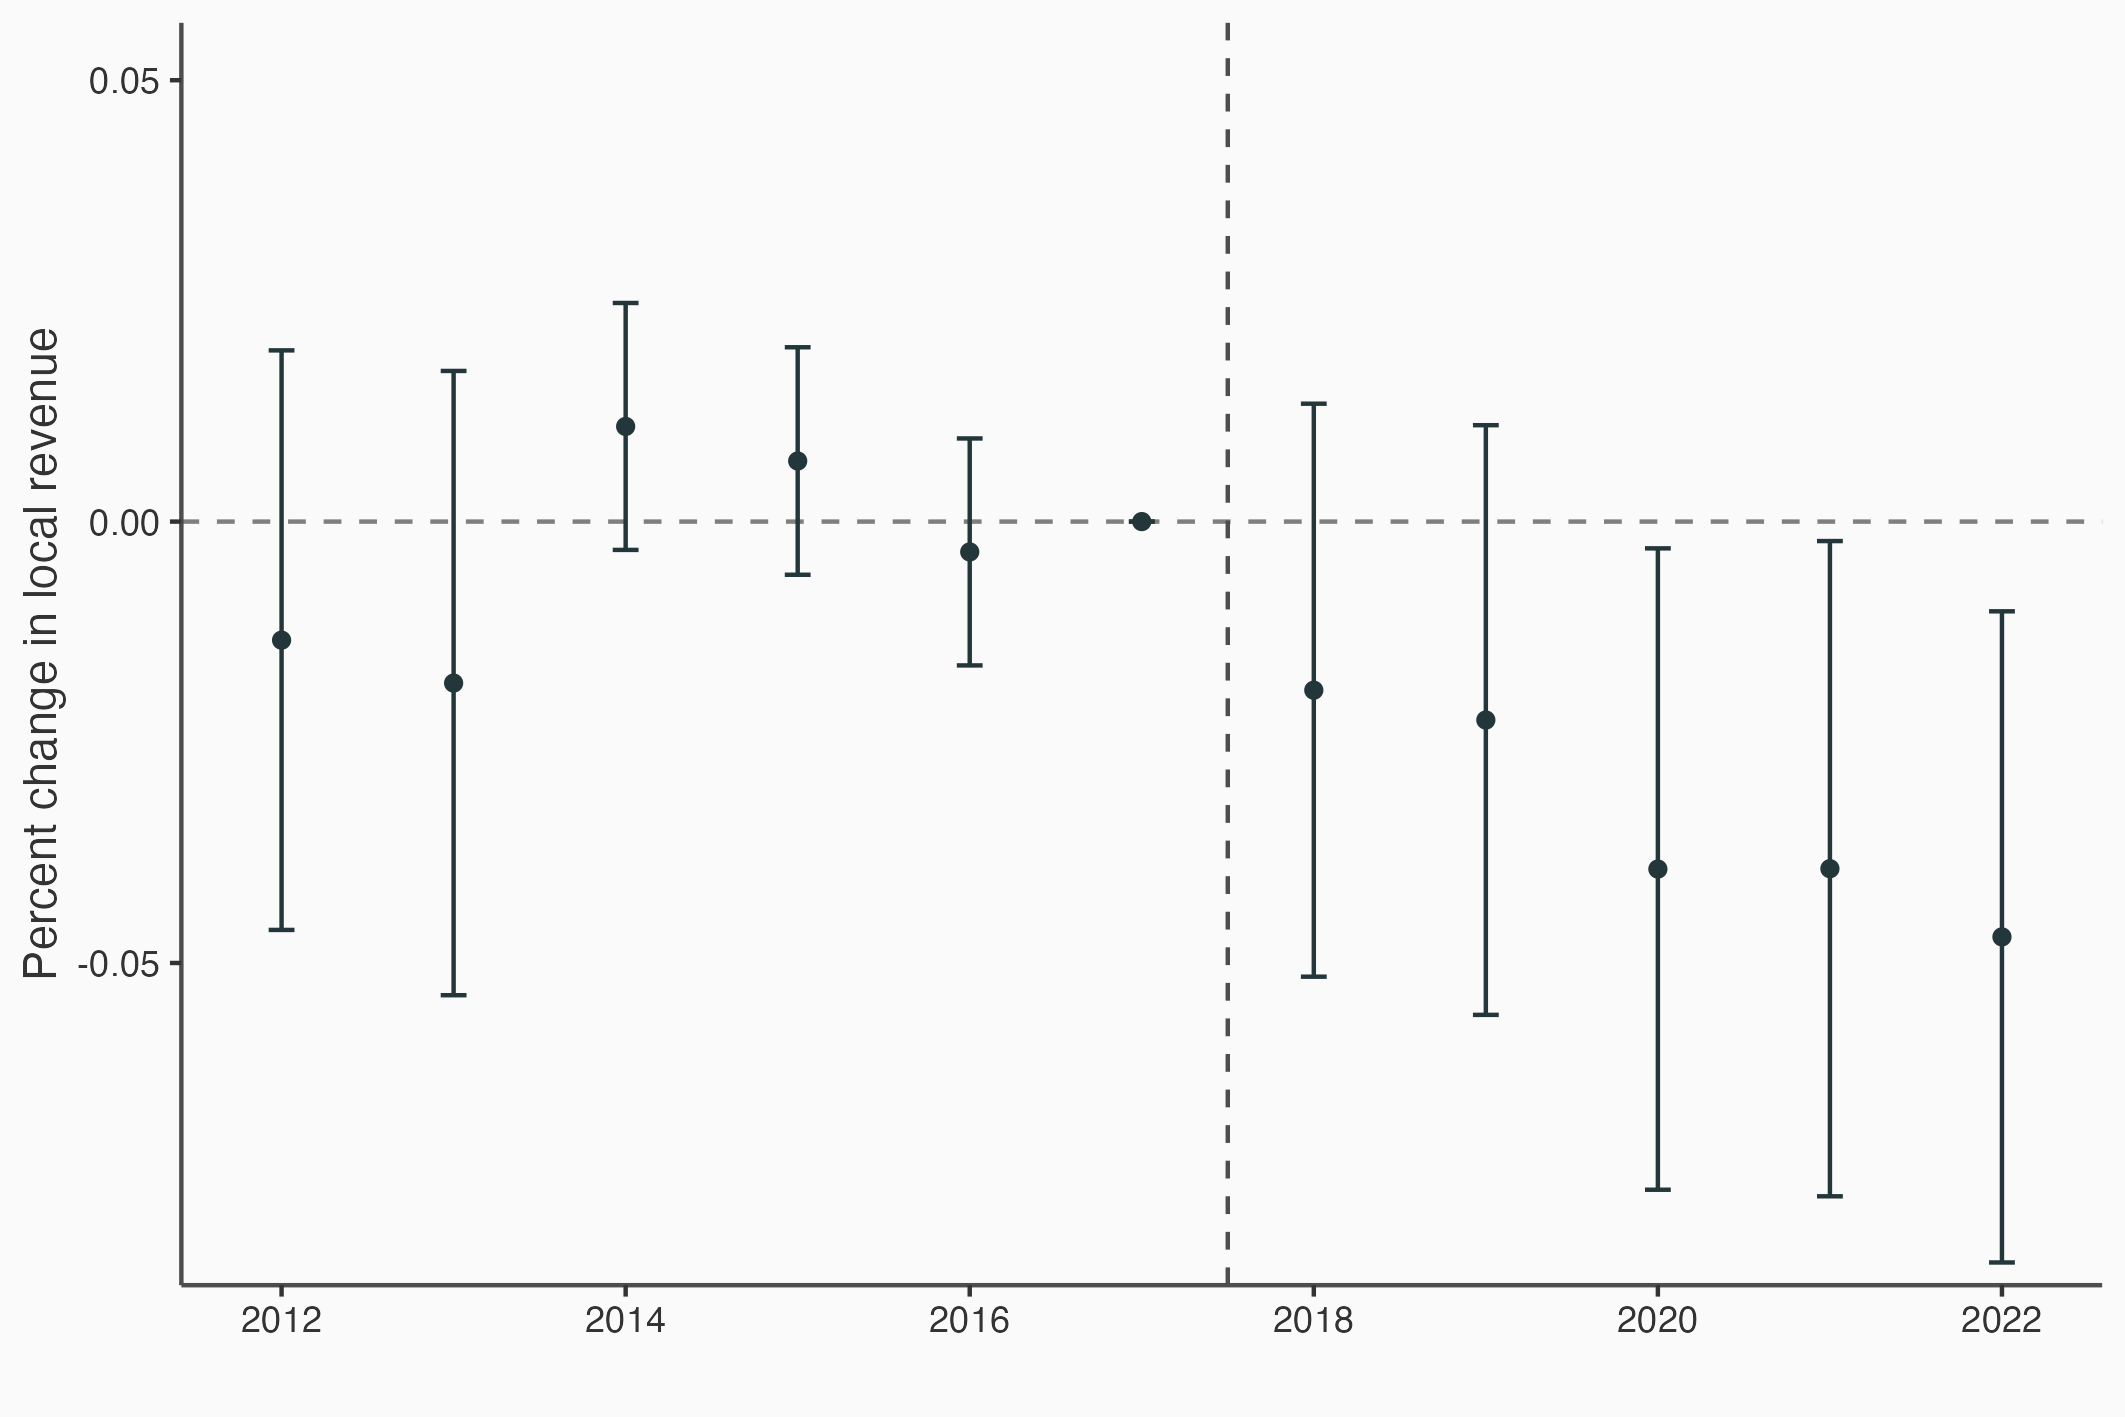
\includegraphics[width=\linewidth]{figures/fig_effective_salt_year_interactions_total_tax.png}
                \label{fig:placeholder}
            \end{figure}
        \end{column}
        \begin{column}{0.4\textwidth}
            \begin{enumerate}
                \item Effect size: Going from the 25th to the 75th percentile of $SALT{it}$ reduces revenue by 6\%.
                \vspace{.15cm}
                \item Perhaps driven by spurious changes in state transfers.
            \end{enumerate}
        \end{column}
    \end{columns}
\end{frame}

\begin{frame}{Only federal transfers and property tax revenues decrease}

    \metroset{block=fill}

    \begin{alertblock}{\textbf{Model}:}
        $$log(y_{it}) = \alpha_i + \beta_t + \alert{\theta_t \cdot SALT_{it}} + \epsilon_{it}$$
    \end{alertblock}
    \vspace{-.3cm}
    \begin{figure}
        \centering
        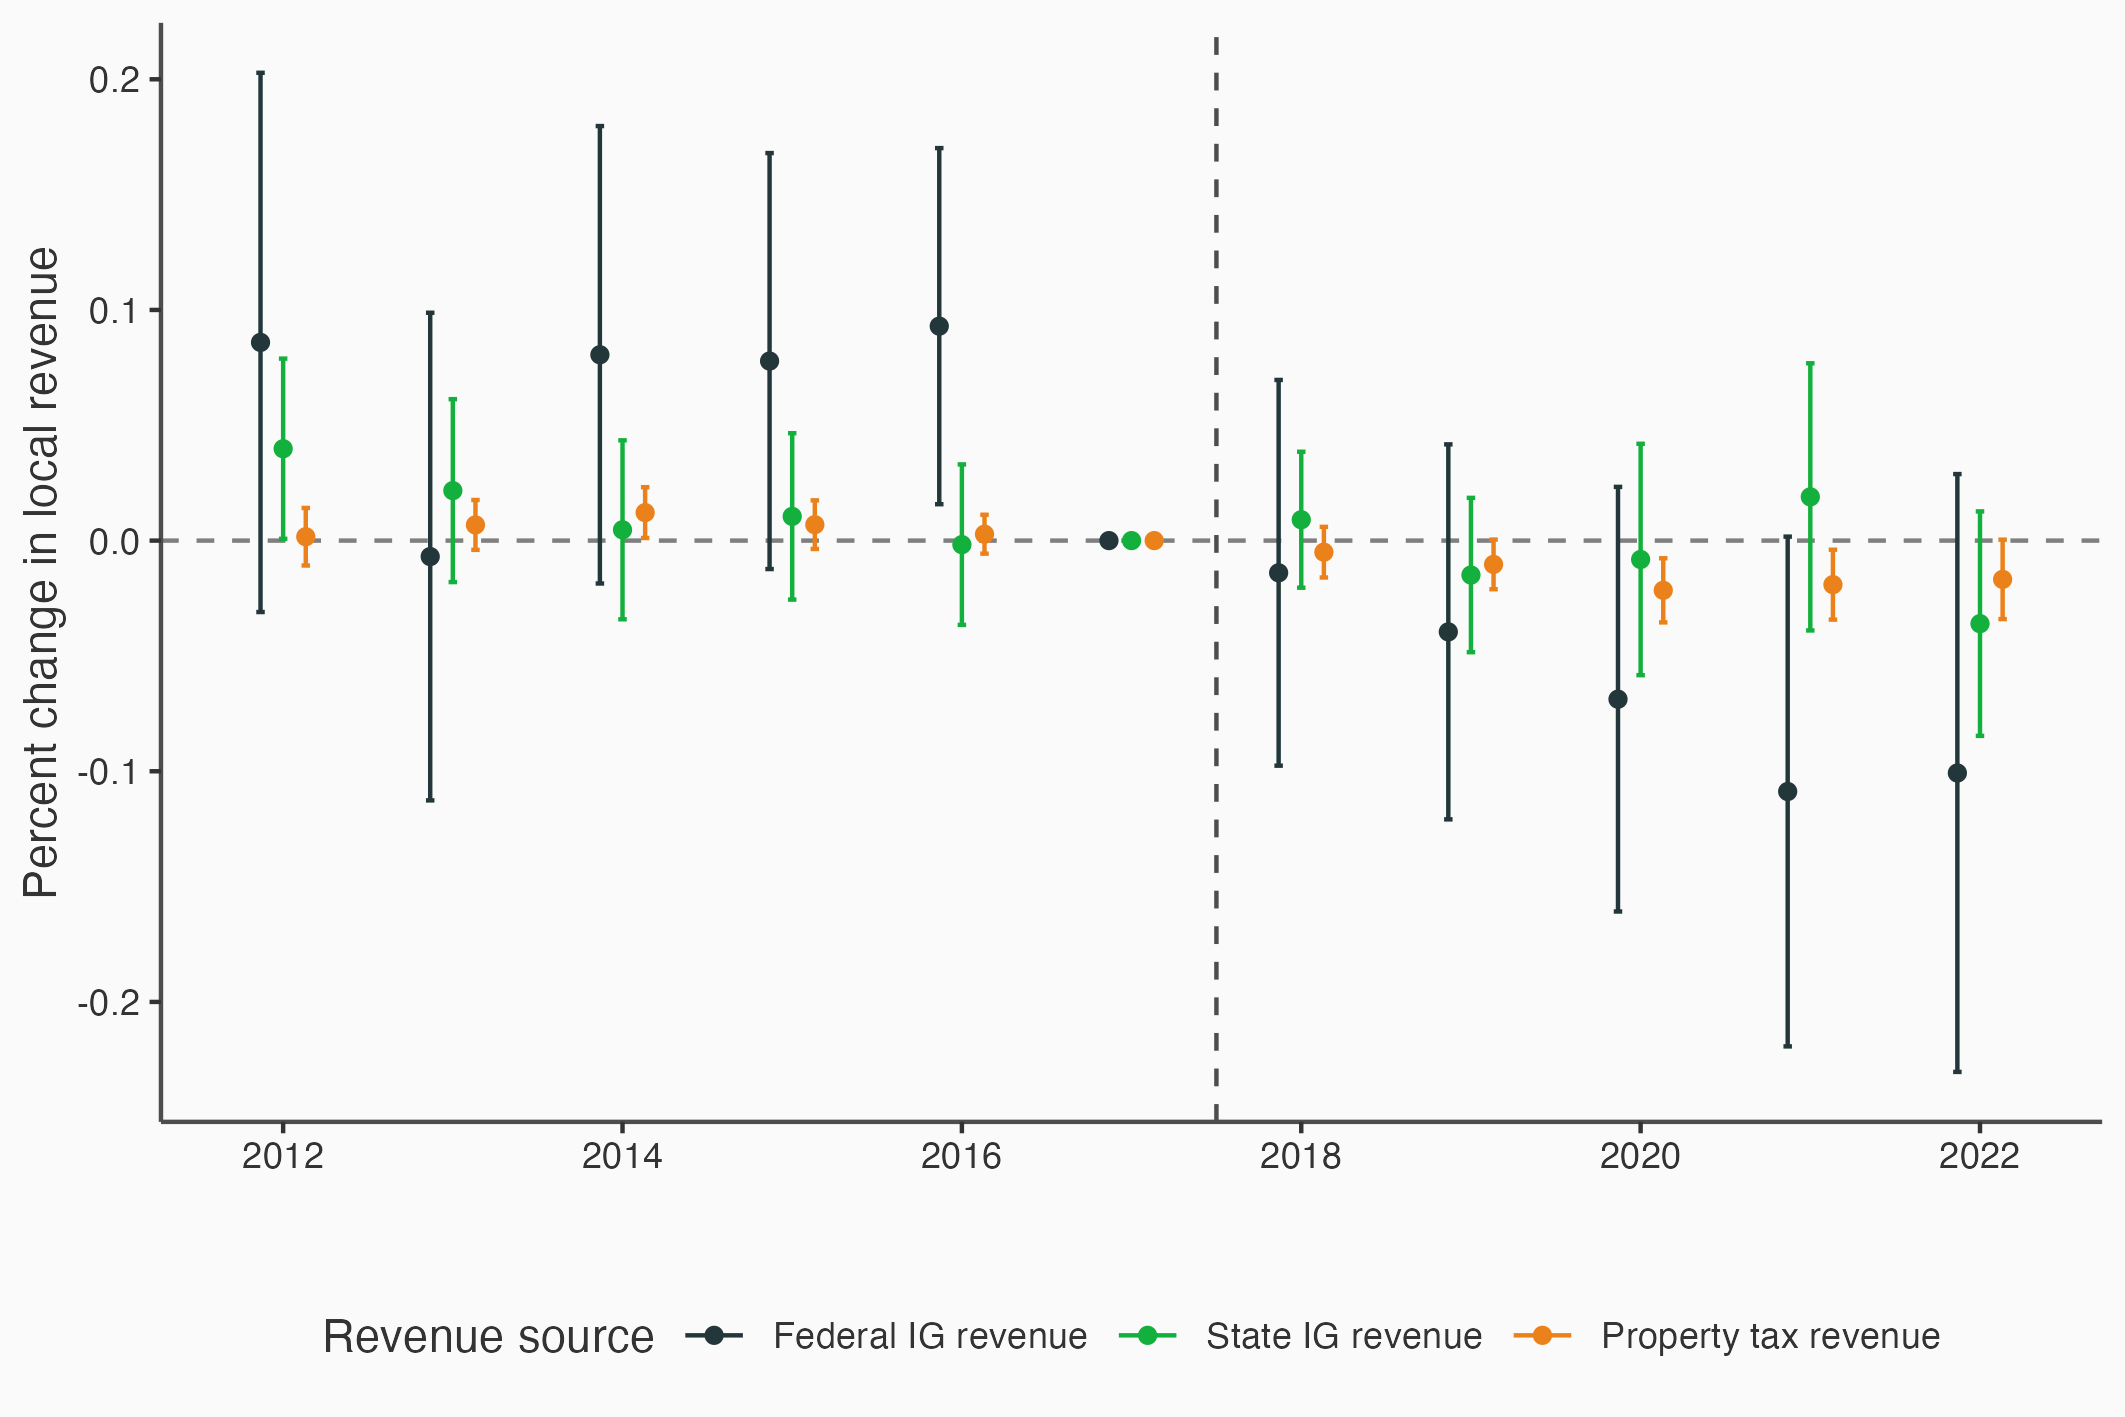
\includegraphics[width=0.65\linewidth]{figures/fig_effective_salt_year_interactions_revenue_sources.png}
        \label{fig:placeholder}
    \end{figure}
\end{frame}

\section{Open Questions}

\begin{frame}{Where to proceed?}
    \begin{enumerate}
        \item IRS data access is unlikely, Census would take a long time, at best. 
        \begin{enumerate}
            \item[$\rightarrow$]Move toward a more structural policy evaluation doable with public data?
        \end{enumerate}
        \item Where to look for local outcomes? School district level data?
        \item Can we make progress on estimating partisan impact with L2 data?
        \item How to think about normative implications?
    \end{enumerate}
\end{frame}

\section[Appendix / old slides]{Appendix / old slides}




\section{Ideal Research Design \& Data}

\begin{frame}{Ideal Research Design}
    \textbf{Two} groups affected by policy:
    \begin{enumerate}
        \item Filers switch from itemizing to taking the standard deduction.
        \begin{itemize}
            \item[$\rightarrow$] \normalsize Changes in the \alert{\textbf{average}} property tax rate.
        \end{itemize}
        \item Filers continuing to itemize, but face the cap.
        \begin{itemize}
            \item[$\rightarrow$] \normalsize Changes in the \alert{\textbf{marginal}} property tax rate.
        \end{itemize}
    \end{enumerate}

    \textbf{Two} possible comparisons:
    \begin{exampleblock}{Never-itemizers vs. Compliers:}
        \begin{itemize}
            \item Selection into treatment if total itemizations between \$6,500 and \$12,000.
            \item Standard approach: \textbf{Diff-in-diff}.
            \item Alternative: IV based on mortgage timing.
        \end{itemize}
    \end{exampleblock}
    
    \begin{exampleblock}{Always-itemizers vs. never-itemizers:}
        \begin{itemize}
            \item Selection into treatment if total itemizations  above \$12,000.
        \end{itemize}
    \end{exampleblock}
\end{frame}

\begin{frame}{Ideal Data}
    \textbf{Data:}
    \begin{itemize}
        \item[(i)] \textbf{Property tax} filings $\rightarrow$ {\color{specialgreen}Corelogic (Cototality)}.
        \item[(ii)] Household \textbf{residence} $\rightarrow$ {\color{specialgreen}Infutor / DataAxle}.
        \item[(iii)] Federal \textbf{income} tax filing $\rightarrow$ \alert{\textbf{????}}
    \end{itemize}

    Could attempt collaborating with IRS, CT department of revenue or imputation schemes.\\
    \vspace{.5cm}

    \begin{block}{\color{specialgreen} Alternative I:}
        \begin{itemize}
            \item New Hampshire has no income and sales tax.
            \item Kink in effective property tax rates at home value of \$10,000.
        \end{itemize}
    \end{block}
    \begin{block}{\color{specialgreen}Alternative II:}
        \begin{itemize}
            \item Exploit border discontinuity in state income taxes.
            \item Shifting itemized totals (= treatment), valid IV if no sorting across state borders.
            \item Relaxed version - sorting not correlated with state income tax rates.
        \end{itemize}
    \end{block}
\end{frame}

\section{Feasible Research Design I: New Hampshire}

\begin{frame}
\frametitle{Research Design}

\begin{columns}[T]
    \begin{column}{0.5\textwidth}
        \centering
        \begin{tikzpicture}[scale=0.8]
            \begin{axis}[
                width=8cm,
                height=6.5cm,
                xlabel={},
                ylabel={},
                xmin=0, xmax=16,
                ymin=0, ymax=1.2,
                xtick={0, 10},
                xticklabels={0, \$10{,}000},
                ytick={0.8},
                yticklabels={$\tau$},
                axis lines=left,
                clip=false,
                scaled x ticks=false,
            ]
            % Y-axis label at top
            \node[anchor=south] at (axis cs:0,1.2) {$E[\tau' | p]$};
            
            % X-axis label at bottom right
            \node[anchor=west] at (axis cs:16,0) {$p$};
            
            % Smooth nonlinear declining curve before jump
            \addplot[thick, specialblue, domain=0:9.9, samples=50] {0.75 - 0.25*(1 - exp(-0.3*x))};
            
            % Jump at p = 10000
            \draw[thick, specialblue, dashed] (axis cs:10,0.53) -- (axis cs:10,0.8);
            
            % Constant line after jump at tau
            \addplot[thick, specialblue, domain=10.1:16, samples=50] {0.8};
            
            % Horizontal dashed line at tau
            \draw[dashed, gray] (axis cs:0,0.8) -- (axis cs:16,0.8);
            
            % Vertical dashed line at p = 10000
            \draw[dashed, gray] (axis cs:10,0) -- (axis cs:10,0.53);
            
            \end{axis}
        \end{tikzpicture}
    \end{column}
    
    \begin{column}{0.5\textwidth}
        \centering
        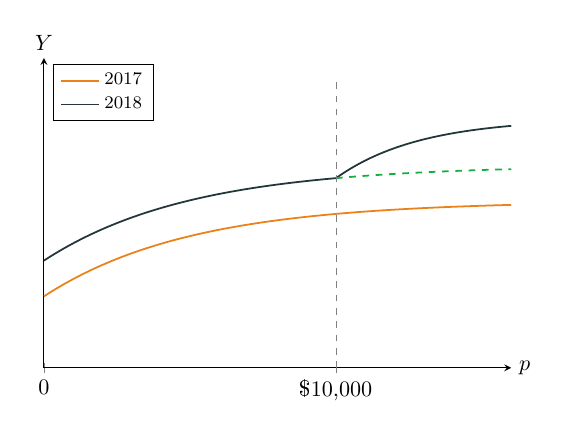
\begin{tikzpicture}[scale=0.8]
            \begin{axis}[
                width=9cm,
                height=6.5cm,
                xlabel={},
                ylabel={},
                xmin=0, xmax=16,
                ymin=0, ymax=1.3,
                xtick={0, 10},
                xticklabels={0, \$10{,}000},
                ytick=\empty,
                axis lines=left,
                clip=false,
                scaled x ticks=false,
                legend style={at={(0.02,0.98)}, anchor=north west, font=\footnotesize},
            ]
            
            % Y-axis label at top
            \node[anchor=south] at (axis cs:0,1.3) {$Y$};
            
            % X-axis label at bottom right
            \node[anchor=west] at (axis cs:16,0) {$p$};
            
            % 2017 smooth nonlinear curve (lower, parallel throughout)
            \addplot[thick, specialorange, domain=0:16, samples=50] {0.3 + 0.4*(1 - exp(-0.2*x))};
            \addlegendentry{2017}
            
            % 2018 smooth nonlinear curve before split
            \addplot[thick, specialblue, domain=0:10, samples=50] {0.45 + 0.4*(1 - exp(-0.2*x))};
            
            % 2018 solid line after split (upper, continues growing)
            \addplot[thick, specialblue, domain=10:16, samples=50] {0.45 + 0.4*(1 - exp(-0.2*10)) + 0.25*(1 - exp(-0.35*(x-10)))};
            
            % 2018 dashed line after split (continues original trend)
            \addplot[thick, specialgreen, dashed, domain=10:16, samples=50] {0.45 + 0.4*(1 - exp(-0.2*x))};
            
            \addlegendentry{2018}
            
            % Vertical dashed line at p = 10000
            \draw[dashed, gray] (axis cs:10,0) -- (axis cs:10,1.2);
            
            \end{axis}
        \end{tikzpicture}
    \end{column}

    \end{columns}

    \vspace{.5cm}
    
    \begin{block}{\alert{\textbf{Identification assumption:}} Parallel trends in $E[Y_{ijt} | p_{ijt}]$.}
        
    \end{block}
    \vspace{-.5cm}
    \hfill{\footnotesize\hyperlink{Math}{\beamergotobutton{Math}}}
    
\end{frame}


\begin{frame}{Corelogic Data}
    I use CoreLogic data from 2014 - 2023.\\
    \vspace{.5cm}
    \metroset{block=fill}
    \begin{block}{\color{specialgreen}Tax records}
        \begin{itemize}
            \item Assessed values and total tax due.
            \item Geocoded based on USPS address API.
            \item About 90 mil. single-family-homes (SFH) per year, 900 mil. observations.
        \end{itemize}
    \end{block}

    \begin{block}{\color{specialgreen}Transaction records}
        \begin{itemize}
            \item Transaction dates and amounts.
            \item Linked based on assessor parcel numbers.
            \item About 90 mil. SFH transactions.
        \end{itemize}
    \end{block}
    
\end{frame}

\begin{frame}{Results}
    \begin{figure}
    \centering
    \caption{Event-Study: Policy exposure in New Hampshire}
    
\includegraphics[width=.7\linewidth]{figures/pctiles.png}
    \label{fig:placeholder}
\end{figure}
\end{frame}

\begin{frame}{Pre-trends}
    \begin{figure}
    \centering
    \caption{Pre-trends: Policy exposure in New Hampshire}
    
\includegraphics[width=.7\linewidth]{figures/pctiles_pretrend.png}
    \label{fig:placeholder}
\end{figure}
\end{frame}

\begin{frame}{Dicussion}
    \begin{block}{\textbf{Effect size:}}
        \begin{itemize}
            \item Property tax payment of \$20,000, assuming marginal federal tax rate of 30\% implies average property tax rate drop of 15\%.
            \item Baseline transaction probability of 5\% implies an elasticity of about 0.66.
        \end{itemize}
    \end{block}

    \begin{block}{\alert{\textbf{Identification assumptions}}}
        \begin{itemize}
            \item Parallel trends in $\mathbb{E}\left[ Y_{ijt} | p_{ijt}\right]$ is avery strong assumption.
            \item Across-state migration during Covid might be confounding estimates.
            \item Vermont or Maine are not valid control groups.
        \end{itemize}
    \end{block}
     
\end{frame}

\section{Feasible Research Design II: Border-RDD}

\begin{frame}{Research Design}

    \begin{block}{\textbf{Idea}}
        \vspace{.1cm}
        \hspace{.25cm}Discontinuity in state income taxes, hence itemized total, at state borders.
    \end{block}
    
    \begin{block}{\alert{\textbf{Concern:}} Sorting}
        \begin{itemize}
            \item Without sorting, itemization rates would jump at borders while other factors are identical.
            \item Discontinuity in effective property tax rates.
        \end{itemize}
    \end{block}
    
    \begin{block}{\color{specialgreen}Relaxed version}
        \vspace{.1cm}
        \hspace{.25cm} Factors affecting transaction probability uncorrelated to state income taxes.
        \begin{itemize}
            \item Test using pre-treatment data.
            \item \textbf{Event-study} of the correlation between state income tax differentials and discontinuity in transaction probability.
        \end{itemize}
    \end{block}
    
\end{frame}

\begin{frame}{Baseline Sorting}
    \begin{figure}
        \centering
        \caption{Sorting along state borders}
        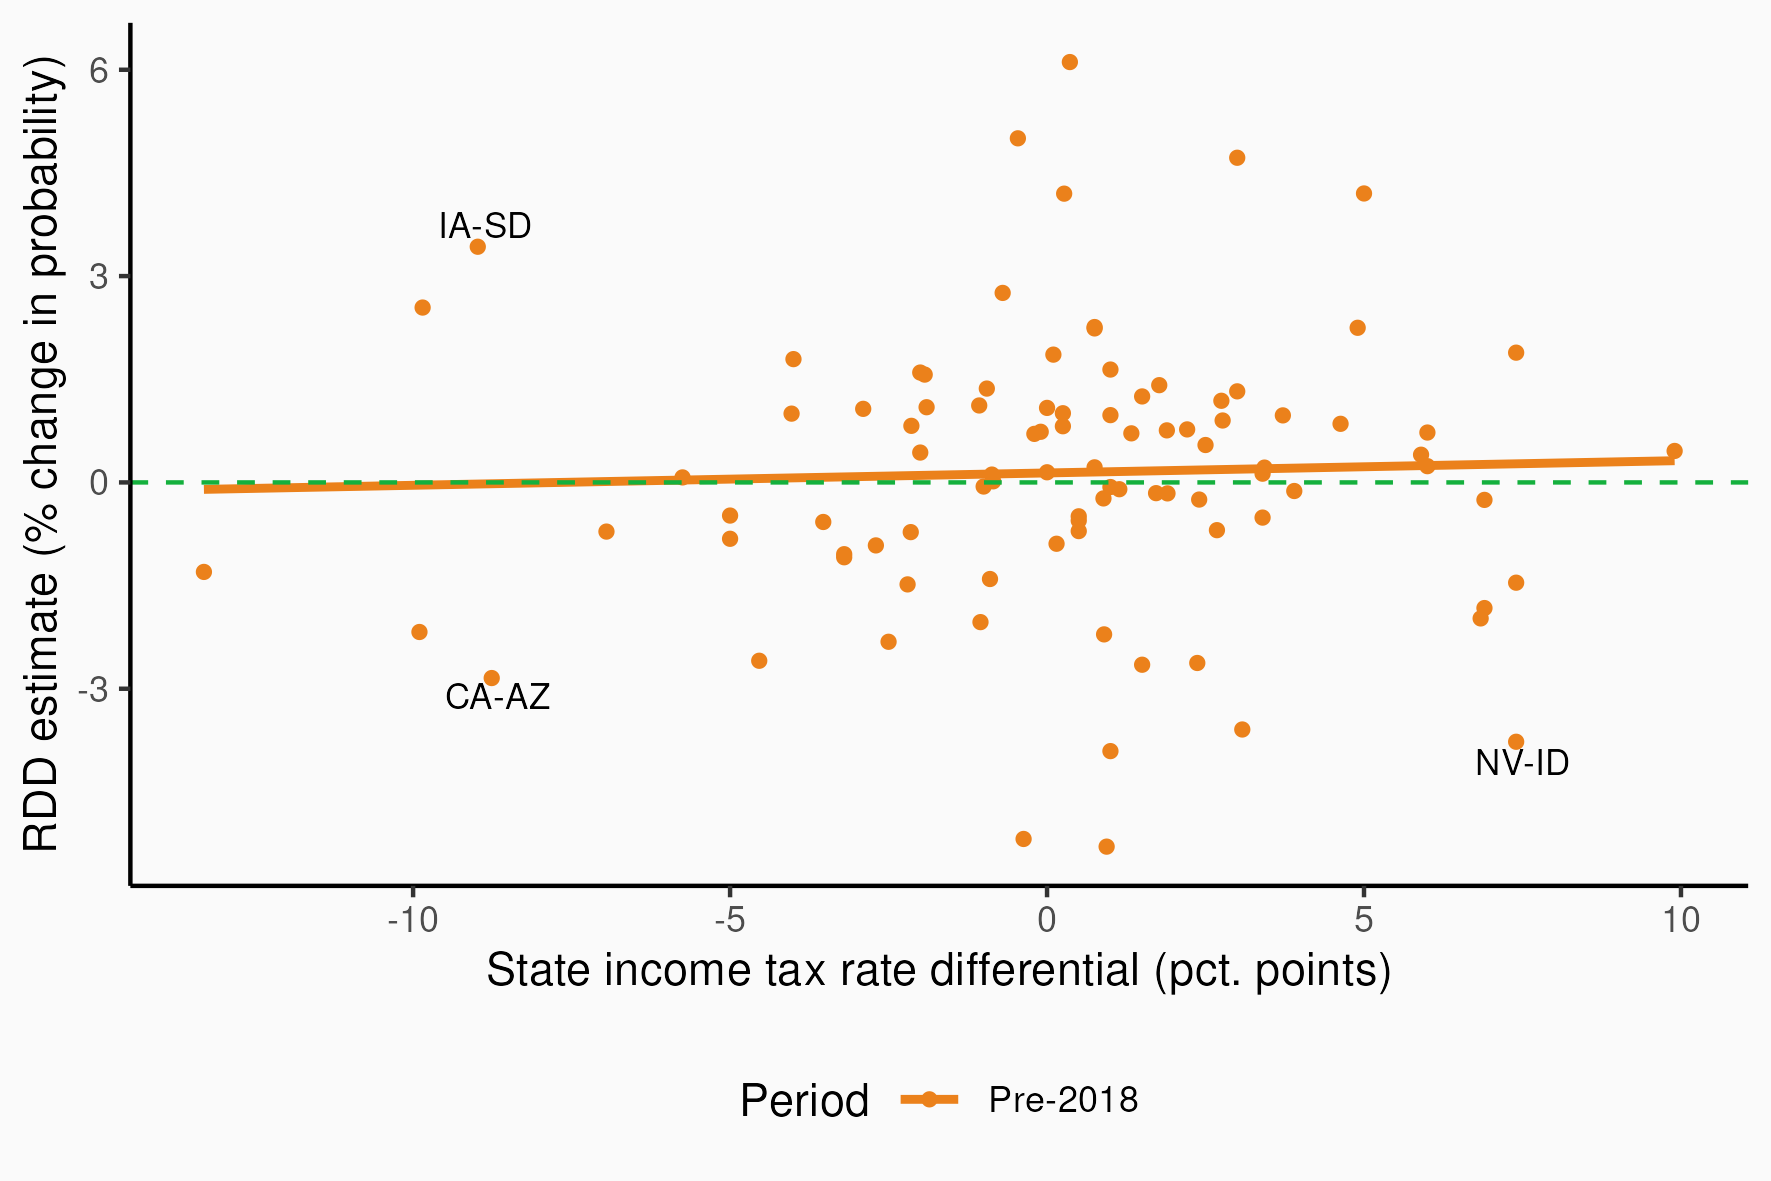
\includegraphics[width=0.7\linewidth]{figures/border_rd_scatter_pre.png}
        \label{fig:placeholder}
    \end{figure}
\end{frame}

\begin{frame}{Results}
    \begin{figure}
        \centering
        \caption{Change in sorting induced by policy}
        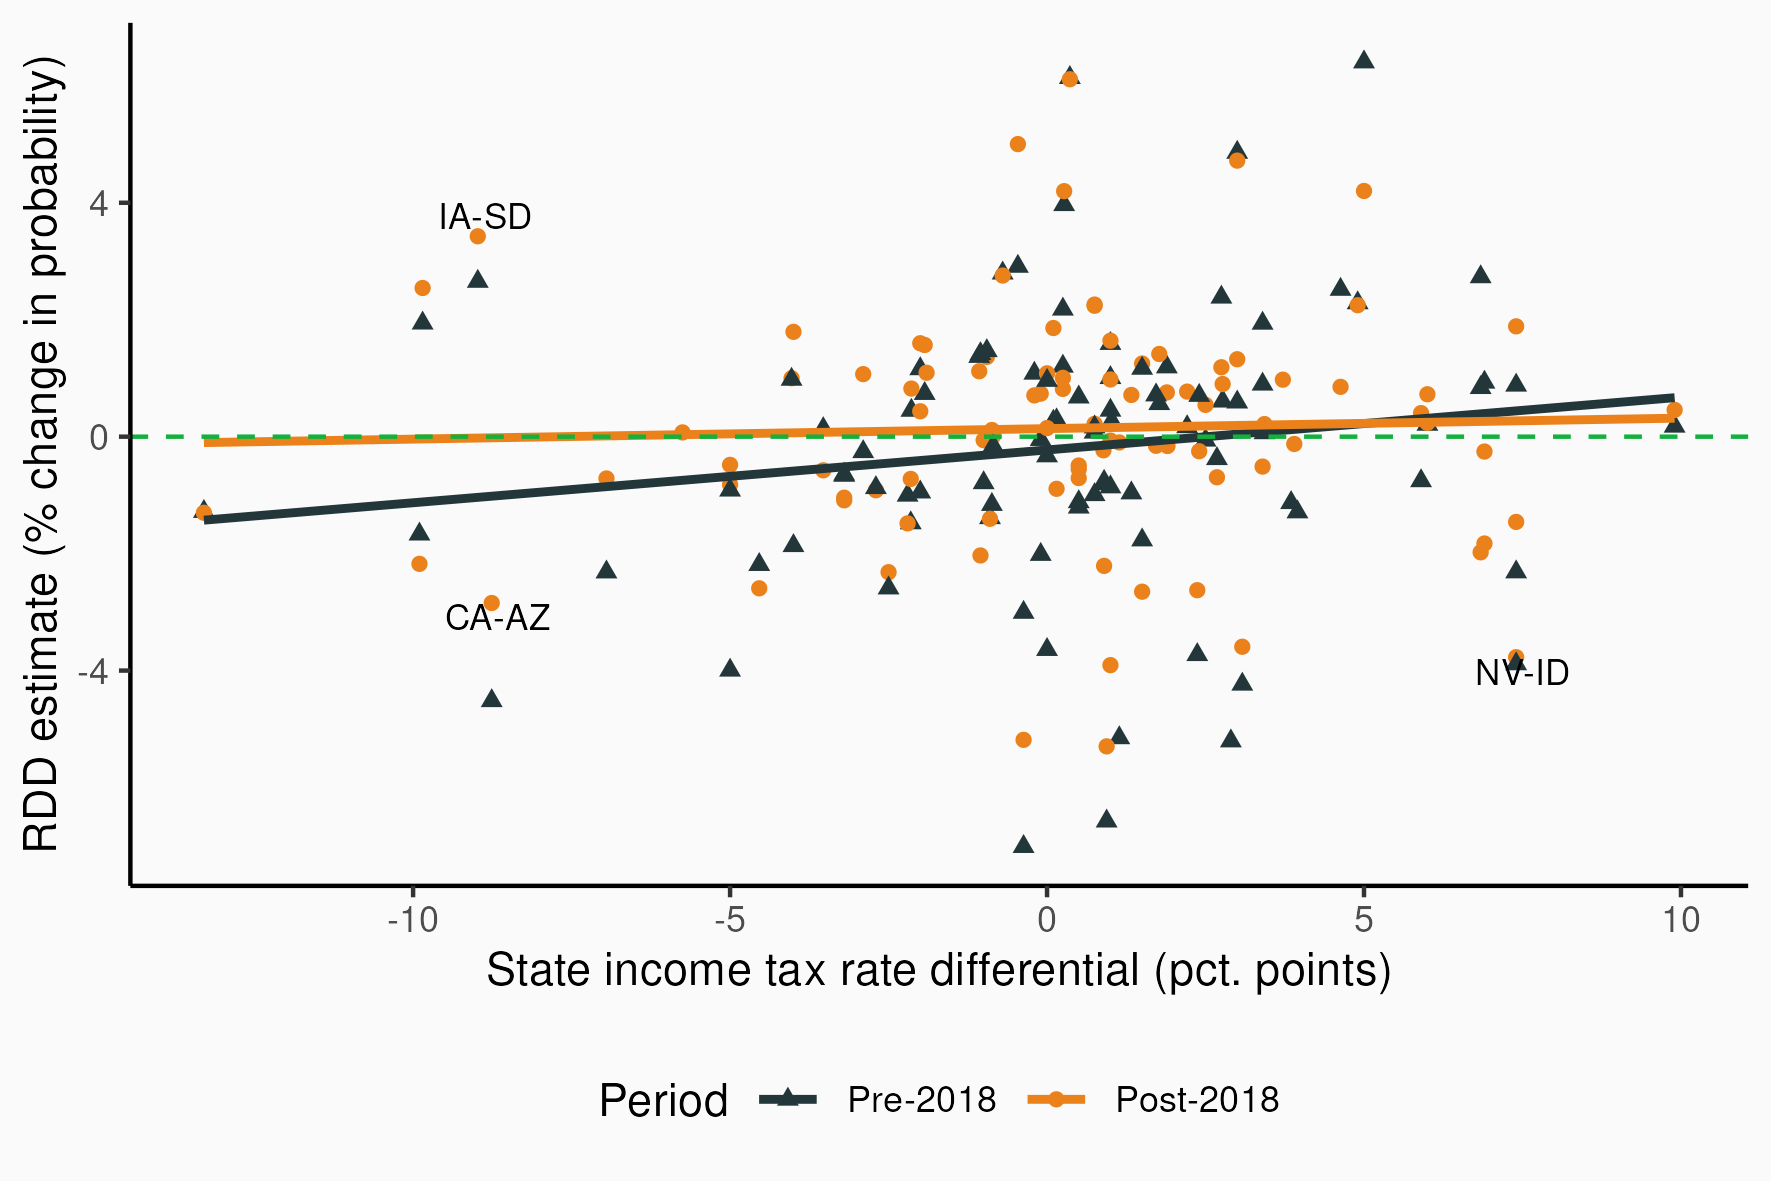
\includegraphics[width=0.7\linewidth]{figures/border_rd_scatter.png}
        \label{fig:placeholder}
    \end{figure}
\end{frame}

\begin{frame}{Pre-Trends}
    \begin{figure}
        \centering
        \caption{Pre-trends in sorting}
        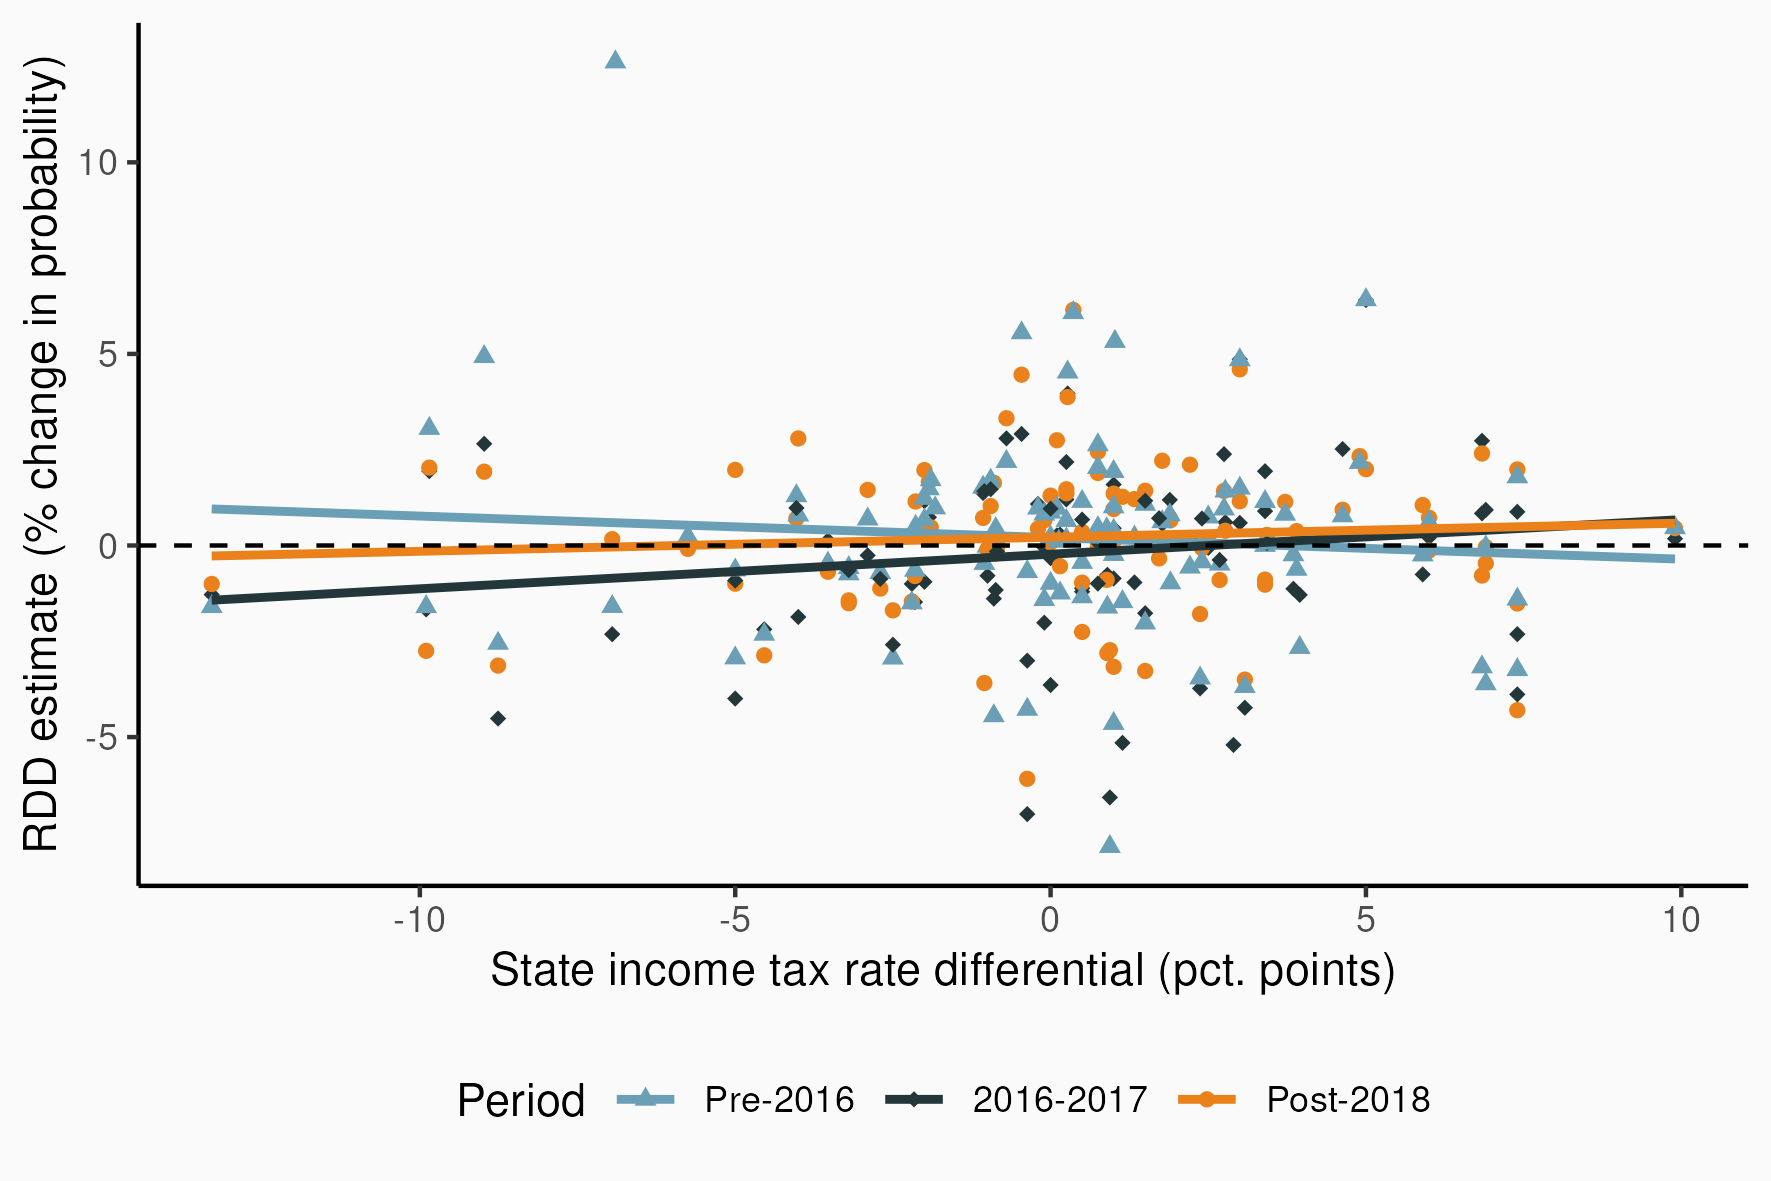
\includegraphics[width=0.7\linewidth]{figures/border_rd_scatter_pretrend.png}
        \label{fig:placeholder}
    \end{figure}
\end{frame}

\begin{frame}{Dicussion}

    \begin{block}{\textbf{Magnitudes}}
        \begin{itemize}
            \item Hard to translate change in \textbf{income-tax}-gradient into transaction elasticity to \textbf{property taxes}.
            \item Inference -  \alert{\textbf{???}}
            \begin{itemize}
                \item 1090 individual border RD estimates.
                \item Estimates correlated across time and across space.
            \end{itemize}
        \end{itemize}
    \end{block}

    \begin{block}{Identification Assumption}
        \begin{itemize}
            \item No pretrends looks questionable.
            \item Treat RDD estimates as panel data?
        \end{itemize}
    \end{block}
    
\end{frame}

\begin{frame}{\color{specialblue}hi}
    \centering \Huge{THANK YOU}
\end{frame}

\begin{frame}[allowframebreaks]{References}

  \bibliography{sample}

\end{frame}



\begin{frame}[label=Math]{Research Design}
\begin{enumerate}
    \item Want to estimate 
        \begin{equation}
            Y_{ijt} = f(\alert{\tau_{ijt}}) + \epsilon_{ijt}
        \end{equation}
        where $Y_{ijt} \in \{0, 1\}$ is a transaction dummy and \alert{$\tau_{ijt}$} the property tax rate for household $i$ in jurisdiction $j$ at time $t$.
    \item Itemization implies
        \begin{equation}
            \alert{\tau_{ijt}} = \tau_{jt}^{nominal} - \mathbb{I}(\text{itemizing})_{ijt}\cdot \mathbb{I}(p_{ijt} \leq  \$10,000)_{ijt} \cdot T^\prime(y_{ijt})
        \end{equation}
        where $p_{ijt}$ is property taxes paid and $y_{ijt}$ is taxable income.
    \item Aggregating, $\mathbb{E}\left[\alert{\tau_{ijt}}\mid p_{ijt}\right]$ has a discontinuity at \$10,000 if $\mathbb{E}\left[\mathbb{I}(\text{itemizing})_{ijt}\cdot T^\prime(y_{ijt}) \mid p_{ijt}\right]$ is smooth in $p_{ijt}$.
    \item If $\mathbb{E}\left[Y_{ijt} \mid p_{ijt} \right]$ does not vary over time, changes after 2017 reveal behavioral responses.
\end{enumerate}
\end{frame}

\end{document}
